\documentclass[11pt,paper=a4,answers]{exam}

\usepackage[a4paper, top=1.5cm, left=2cm, right=2.4cm, bottom=2cm, headsep=.5\baselineskip]{geometry}
\usepackage[utf8]{inputenc}
\usepackage{graphicx,lastpage}
\usepackage{censor}
\usepackage{tabularx} 
\usepackage[normalem]{ulem}
\usepackage{caption}

% Zensierte wörter werden durch einen Unterstrich ersetzt
\censorruledepth=-.2ex
\censorruleheight=.1ex
\hyphenpenalty 10000

\flushbottom

% Dicke des Striches nach dem Header
\renewcommand\ULthickness{2pt}  
% Abstand zwischen Header und Unterstrich 
\setlength\ULdepth{1.5ex}
% Einfacher Zeilenabstand
\renewcommand{\baselinestretch}{1}
\pagestyle{empty}


%%%%%%%%%%%%%%%%%%%%%%%%%%%%%%%%%%%%%%%%%%%%%%%%%%%%%%%%%%%%%%%
% UPDATE EACH SEMESTER
\newcommand{\semester}{WS23}
\newcommand{\bearbeitungszeit}{1h}
\newcommand{\treffpunkt}{Süd-Ende Bota}
\newcommand{\treffpunktinline}{das Süd-Ende des Botas}
%%%%%%%%%%%%%%%%%%%%%%%%%%%%%%%%%%%%%%%%%%%%%%%%%%%%%%%%%%%%%%%

\pagestyle{headandfoot}
\headrule
\newcommand{\continuedmessage}{%
\ifcontinuation{\footnotesize Question \ContinuedQuestion\ continues\ldots}{}%
 }
\runningheader{\footnotesize Stadtrallye}
{\footnotesize Fachschaften Informatik \& Kognitionswissenschaft}
{\footnotesize Seite \thepage\ von \numpages}
\footrule
\footer{\footnotesize Stadtrallye \semester}
{}
{\ifincomplete{\footnotesize Question \IncompleteQuestion\ continues
on the next page\ldots}{\iflastpage{\footnotesize End Of File}{\footnotesize Auf der Rückseite geht's weiter\ldots}}}

% Überschreibe den Stil der Fragen
\let\q\questions
\renewenvironment{questions}{
	\begin{q}
		\pointsinrightmargin
		\marginpointname{\ Pkt}
		\bracketedpoints }{
	\end{q}}

%\crefname{figure}{figure}{figures}
%\crefname{question}{question}{questions}
%==============================================================
\begin{document}
	
% Minipage für das icon auf der linken Seite
\noindent
\begin{minipage}[l]{.1\textwidth}
\noindent
\includegraphics[width=1.5\textwidth]{graphics/denker}
\end{minipage}
% Minipage für den Inhalt des Titels.
% Breite sind 0.8 * textwidth, so dass der Text trotz Icon mittig platziert wird.
\begin{minipage}{.8\textwidth}
\begin{center}
{\large \bfseries Fachschaft Informatik Tübingen \\
\bfseries Fachschaft Kognitionswissenschaft Tübingen \\
\vspace{0.5mm}
\Large Stadtrallye \semester}
%  \vspace{0.5cm}
\end{center}
\end{minipage}
% Hinzufügen des Kognilogos als Minipage auf der rechten Seite
\hspace{-12mm}
\begin{minipage}[r]{.1\textwidth}
\noindent
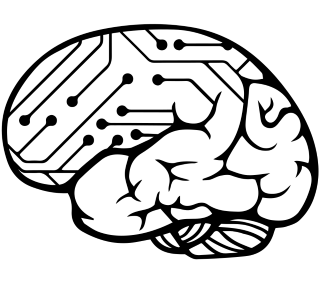
\includegraphics[width=1.5\textwidth]{graphics/kogni}
\end{minipage}
\par
%Kleiner Abstand zwischen Bild und Textzeile.
\vspace{0.5cm}
\noindent
\uline{Gruppe:\hspace{2cm} \hfill Bearbeitungszeit: \bearbeitungszeit   \hfill     Treffpunkt: \treffpunkt}
%Kleiner Abstand zwischen Header und Fragen
\vspace{0.5cm}\\
Findet euch in den zuvor eingeteilten Gruppen mit je \textbf{6 ($\pm$1) Person} zusammen. Ihr habt
\textbf{\bearbeitungszeit} Zeit um so viele Aufgaben wie möglich zu lösen und
fleißig Punkte zu sammeln. Der \textbf{Treffpunkt ist \treffpunktinline}. Wird
die Bearbeitungszeit überschritten muss ab einer Verspätung von 5 Minuten mit einem Punktabzug von 2 Punkten pro Minute gerechnet werden. Für jede Minute früher gibt es zudem einen Bonuspunkt.
Anschließend kann der Abend beim Spieleabend der Psychologen am Psychologischen Institut enden. 

\section*{Stationsaufgaben}
\subsection*{Bota}
\begin{questions}
\question[10-50] Baut eine Menschenpyramide. \\
Dabei gibt es 10 Punkte pro Ebene bzw. 50 Punkte bei 4 Ebenen. Ihr dürft Euch für die Bewältigung dieser Aufgabe mit anderen Gruppen zusammentun, aber brecht Euch bitte nichts!

\end{questions}

\subsection*{Altstadt}
\begin{questions}
\question[10-25] Inszeniert auf dem Marktplatz am Rathaus eine Szene aus eurem Lieblingsfilm. \\
Dabei gibt es 10 Punkte für ein Foto und 25 Punkte für ein Video der Szene.
\question[10] Sucht euch im Rathaus einen Flyer aus. \\
Bringt den Flyer mit zum Treffpunkt und überzeugt euren Betreuer von der im Flyer angepriesenen Sache.
\question[10] Ein berühmter Dichter war hier dichter als ihm guttat. \\
Macht ein Foto mit seinem Gedenkschild nahe der Stiftskirche am Holzmarkt.

\end{questions}

\subsection*{Neckarbrücke}
\begin{questions}
	\question[10] Stellt das Titanic-Bild nach (Beweisfoto).
	\question[10] Setzt Euch auf die Steinmauer und macht ein Touri-Foto. 
	\question[5] Stoßt an der Steinmauer mit einem Passanten an.
	\question[1 Pkt pro Ente auf dem Foto + 10] Macht ein Foto auf dem Stocherkahnsteg am Hölderlinturm

\end{questions}

\subsection*{Schloss Hohentübingen}
\begin{questions}
	\question[10] Genießt den Ausblick über Tübingen (Foto)
	\question[10] Führt den Römer an der Nase herum (Foto)
	\question[10] Der Kern des Menschen wurde hier entdeckt.\\
Findet das Labor, macht ein Bild und zeigt darauf eure Liebe zur Wissenschaft.

\end{questions}

\newpage

\section*{Aufgaben für den Weg}
\subsection*{Jäger \& Sammler}
\begin{questions}
	\question[5] Macht ein Foto vom Mann mit der Kinderbrille
	\question[5] Wo befindet sich der eiserne Mann auf dem Fahrrad? Beweisbild
	\question[5] Findet eine wirklich 	schwere Lektüre und tätigt einen Schnappschuss von ihr
	\question[5] Zeigt uns das Foto einer äußerst schwäbischen Bank
	\question[je 1] Fotografiert eine schnelle Essgelegenheit
	\question[10] Sammelt 5 unterschiedliche Kronkorken
	\question[20] Sammelt 20 Unterschriften verschiedener Personen auf einem Bauch
	
\end{questions}

\subsection*{Hochkultur}
\begin{questions}
	\question[10] Schreibt ein Liebesgedicht für Tübingen und tragt es eurem Betreuer vor
	\question[20] Performt eine Choreografie zum Klassiker "Tübingen warum bist du so hügelig"
	\question[Schnupfen + 50] Geht im Neckar baden (min. 50\% der Körperfläche müssen bedeckt sein

\end{questions}
\vspace{15mm}
\begin{figure}[ht]
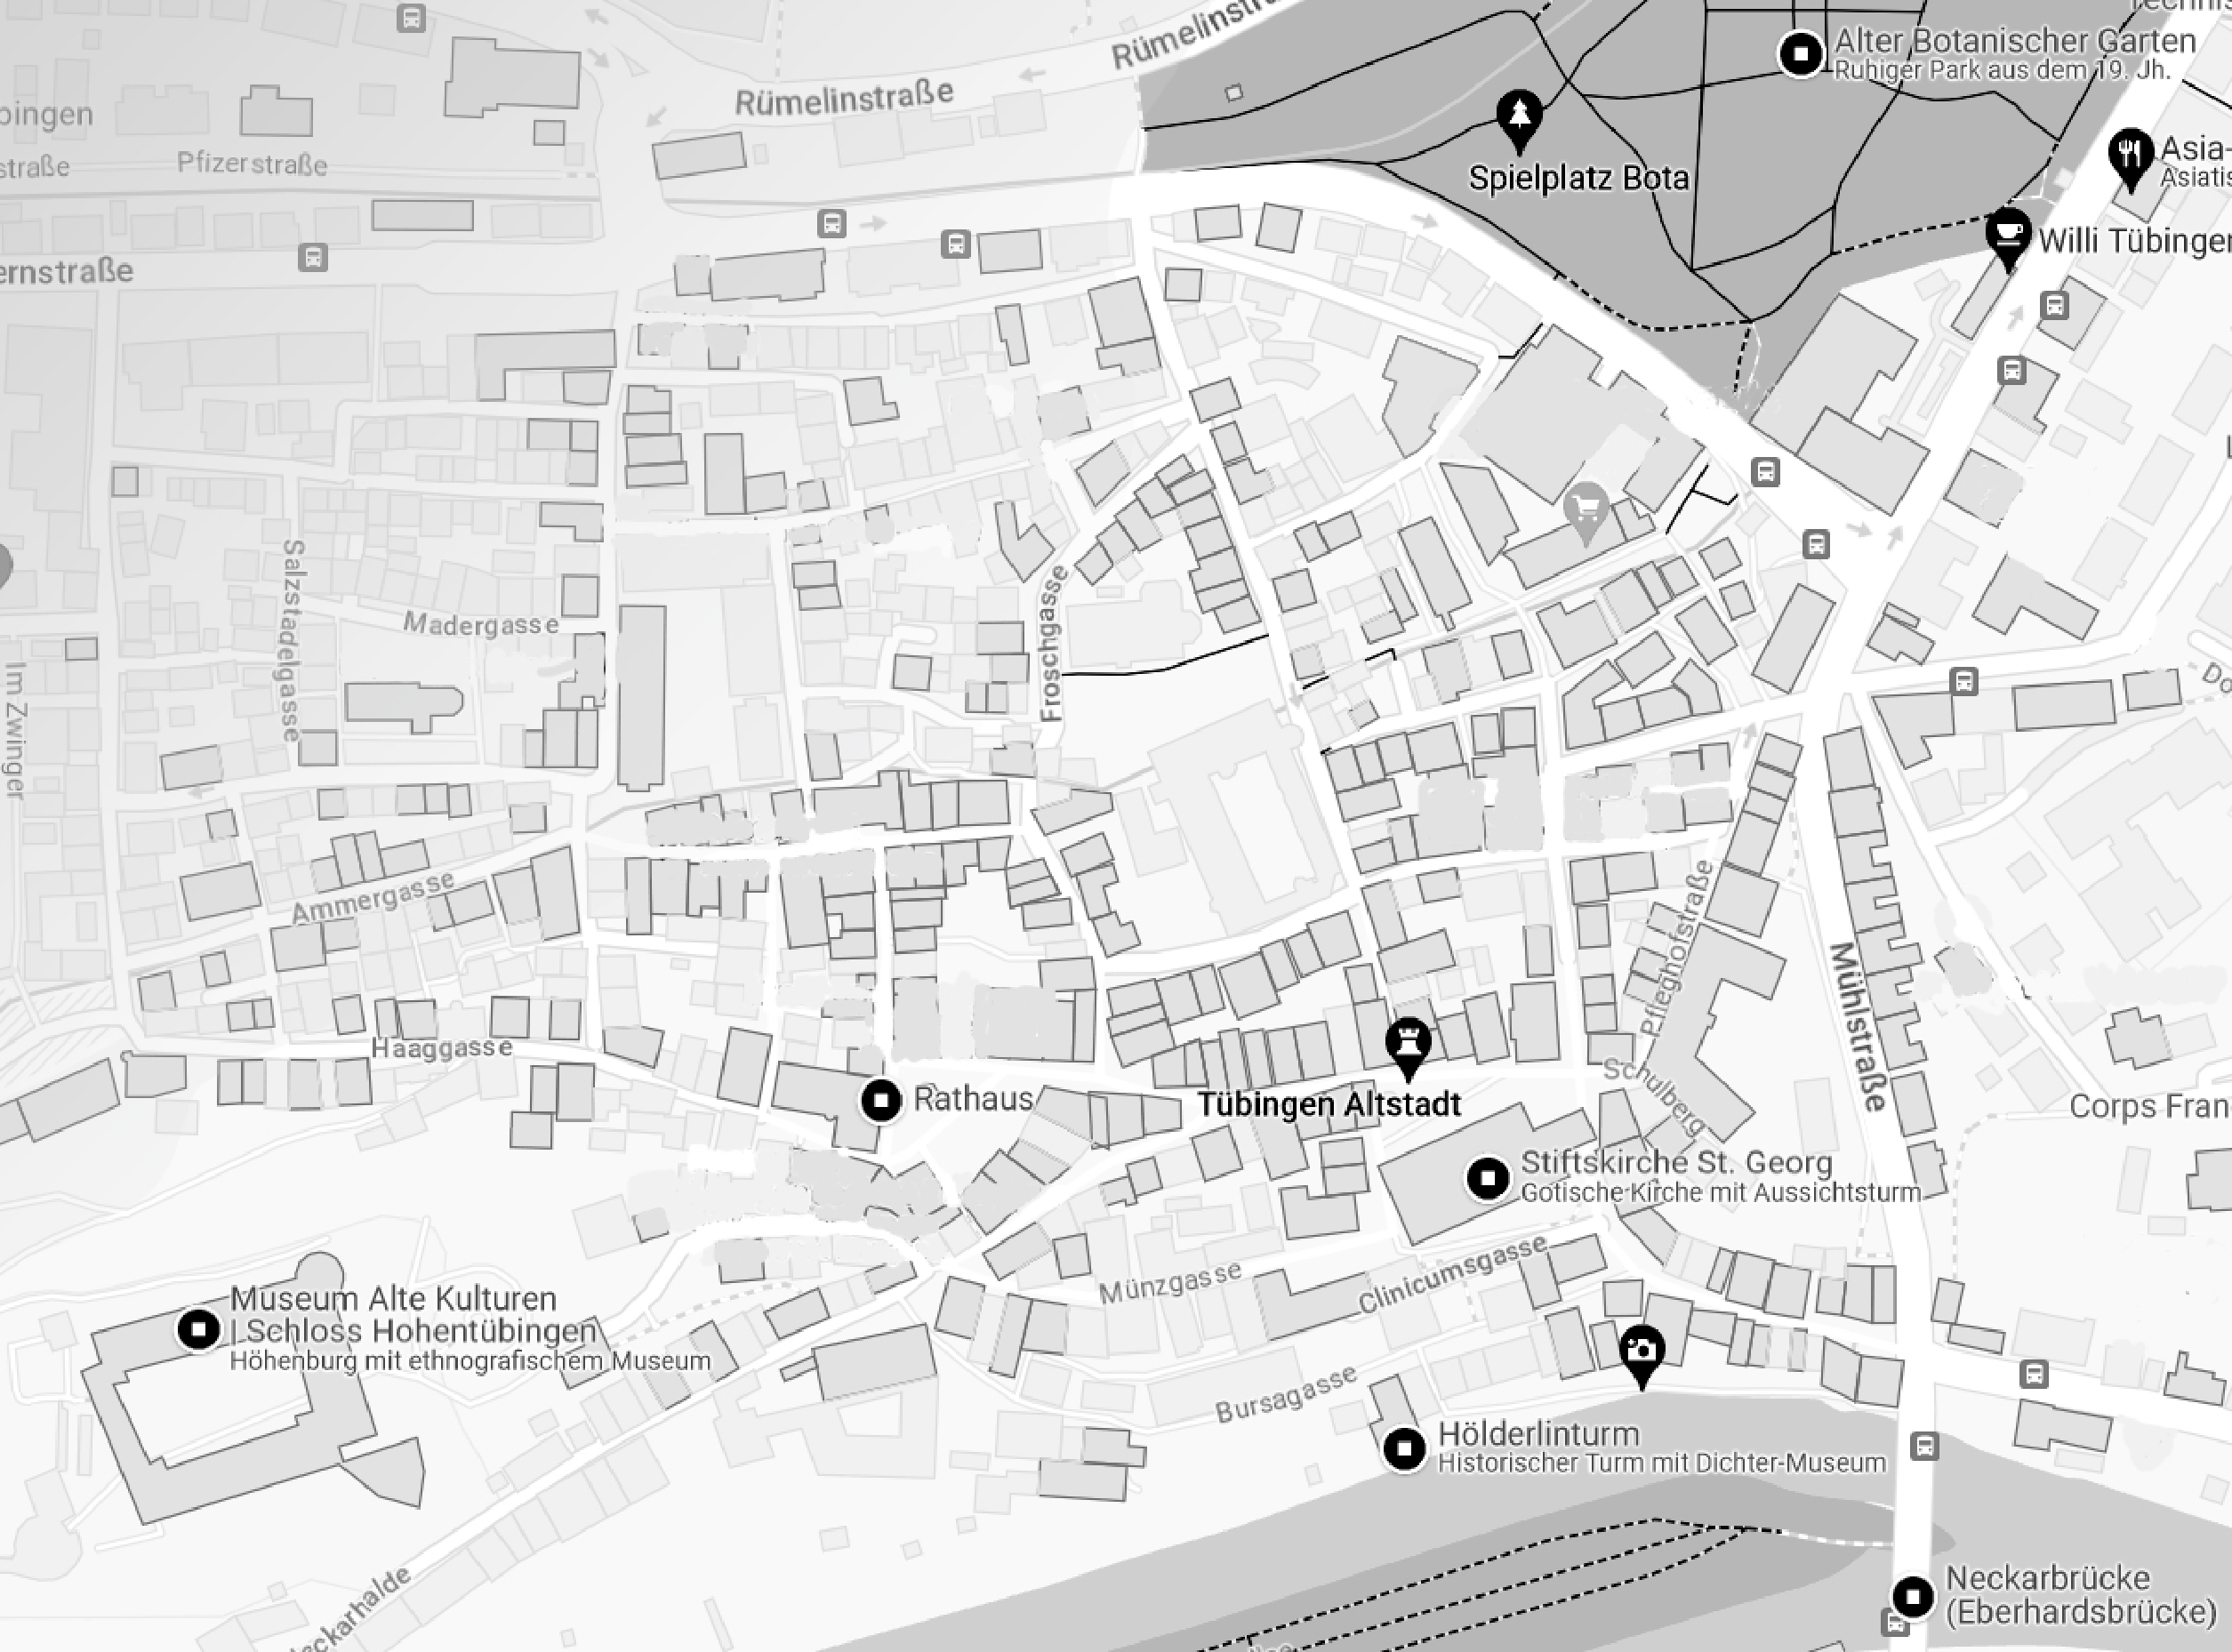
\includegraphics[width=\textwidth]{graphics/Karte_Stationen}
\captionsetup{labelformat=empty}
\caption{Damit Ihr Euch nicht verlauft ist hier eine Karte mit den wichtigsten Standorten}
\end{figure}
 
\end{document} 



% ************************** Old Version below ****************************
%\section*{Sammelaufgaben}
%	Sammelt folgende Dinge und bringt sie zu uns:
%	\begin{questions}
%		\question[10] 5 Kronkorken von verschiedenen Biersorten
%		\question[10] 1 Glückskeks
%		%\question[15] Die Visitenkarte eines Anwaltes
%		% Anwälte wirkten zuletzt genervt
%		\question[25] 25 Unterschriften auf einem Bauch eurer Wahl
%		%\question[5] Ein Kassenzettel aus dem Alnatura
		
%	\end{questions}

%\section*{Gruppenfotos}
%	Macht Gruppenfotos an folgenden Orten/ mit folgenden Personen:
%	\begin{questions}
%		\question[6+6] Vor 6 verschiedenen Dönerbuden (für deren Stempel worauf auch immer +1 Punkt)
%		\question[5] Vor 5 Gebäuden des StuWe 
%		\question[5] Macht ein Bild beim Kartenterminal in der Unibib
%		\question[10] Gruppenfoto in einem Baum
%		\question[100] Mit Boris Palmer
%		\question[10] Mit Polizisten in Uniform
%		\marginpointname{} 
%		\question[$n^2$ Pkt pro Ebene] Bildet eine menschliche Pyramide im alten Bota
		%\question[2 Pkt pro Person auf dem Foto] Auf einer WG-Party
	
%	\end{questions}

%\section*{Aktionsaufgaben}
%	Folgende Aufgaben müssen von mindestens einer Person aus eurer Gruppe erfüllt
%	werden. Die Person muss auf dem Beweisfoto zu sehen sein.
	
%	\begin{questions}
%		\question[5] Macht ein Titanic-Bild auf der Neckarbrücke
%		\question[5] Findet ein Fahrrad, das mit Blumen geschmückt ist
%		\question[20] Tanzt die Choreo aus dem Refrain von \textbf{Tübingen warum bist du so hügelig} (Video)
%		\question[50] Geht Baden im Neckar (Mindestens 50\% des Körper muss mit Wasser bedeckt sein)
		%\question[5] Esst eine Portion Käs' Spätzle
%		\question[10] Schreibt ein Liebesgedicht für Tübingen und tragt es am Ende der Rallye vor
		%\question[5] Trinkt ein Bier (0,5l) auf Ex (Video)
%		\marginpointname{}
%		\question[5 Pkt pro Ort] Findet folgende Orte:
		
%	\end{questions}
%\ \\
%\noindent
%\begin{tabularx}{19cm}{XX}
%	\includegraphics[width=7.5cm]{graphics/suche_1} & 
%	\includegraphics[width=7.5cm]{graphics/suche_2} \\ 
%	\includegraphics[width=7.5cm]{graphics/suche_3} & 
%	\includegraphics[width=7.5cm]{graphics/suche_4} \\ 
%	\includegraphics[width=7.5cm]{graphics/suche_5} & 
%	\includegraphics[width=7.5cm]{graphics/suche_6}
%\end{tabularx}